\begin{sidewaysfigure}
  \begin{center}
    \resizebox{\textwidth}{!}{%
    \begin{tikzpicture}
      \node (n0) at (0,0) {\huge\textbullet};
      \node (n1) at (0.3,0) {\huge\textbullet};
      \node (n3) at (2.3,0) {\huge\textbullet};
      \node (n5) at (2.6,0) {\huge\textbullet};
      \node (n6) at (7.6,0) {\huge\textbullet};
      \node (n7) at (11.6,0) {\huge\textbullet};
      \node (n8) at (11.9,0) {\huge\textbullet};
      \node (n10) at (13.9,0) {\huge\textbullet};
      \node (n12) at (14.2,0) {\huge\textbullet};
      \node (n13) at (19.2,0) {\huge\textbullet};
      \node (n14) at (24.2,0) {\huge\textbullet};
      \node (n15) at (24.5,0) {\huge\textbullet};
      \node (n17) at (26.5,0) {\huge\textbullet};
      \node (n19) at (26.8,0) {\huge\textbullet};
      \node (n20) at (31.8,0) {\huge\textbullet};
      \node (n21) at (37.8,0) {\huge\textbullet};
      \node (n22) at (38.1,0) {\huge\textbullet};
      \node (n25) at (40.1,0) {\huge\textbullet};
      \node (n26) at (40.4,0) {\huge\textbullet};
      \node (n27) at (41.4,0) {\huge\textbullet};
      \node (n28) at (41.7,0) {\huge\textbullet};
      \node (n30) at (44.7,0) {\huge\textbullet};
      \node (n31) at (47.7,0) {\huge\textbullet};
      \node (n32) at (48,0) {\huge\textbullet};
      \node (n34) at (50,0) {\huge\textbullet};
      \node (n36) at (50.3,0) {\huge\textbullet};
      \node (n37) at (53.5,0) {\huge\textbullet};
      \node (n40) at (53.8,0) {\huge\textbullet};
      \node (n43) at (55.8,0) {\huge\textbullet};
      \node (n45) at (58.8,0) {\huge\textbullet};
      \node (n47) at (59.1,0) {\huge\textbullet};
      \node (n49) at (63.1,0) {\huge\textbullet};
      \node (n50) at (63.4,0) {\huge\textbullet};
      \node (n52) at (65.4,0) {\huge\textbullet};
      \node (n55) at (65.7,0) {\huge\textbullet};
      \node (n56) at (67.7,0) {\huge\textbullet};
      \node (n58) at (68,0) {\huge\textbullet};
      \node (n60) at (71,0) {\huge\textbullet};
      \node (n62) at (74,0) {\huge\textbullet};
      \node (n64) at (74.3,0) {\huge\textbullet};
      \node (n66) at (77.3,0) {\huge\textbullet};
      \node (n68) at (80.3,0) {\huge\textbullet};
      \node (n69) at (80.6,2) {\huge\textbullet};
      \node (n70) at (85.6,2) {\huge\textbullet};
      \node (n71) at (90.6,2) {\huge\textbullet};
      \node (n72) at (90.9,2) {\huge\textbullet};
      \node (n74) at (93.9,2) {\huge\textbullet};
      \node (n76) at (94.2,2) {\huge\textbullet};
      \node (n77) at (98.2,2) {\huge\textbullet};
      \node (n78) at (102.2,2) {\huge\textbullet};
      \node (n79) at (102.5,2) {\huge\textbullet};
      \node (n81) at (104.5,2) {\huge\textbullet};
      \node (n38) at (104.8,2) {\huge\textbullet};
      \node (n39) at (109.8,2) {\huge\textbullet};

      \node (n41) at (53.8,2) {\huge\textbullet};
      \node (n42) at (55.8,2) {\huge\textbullet};
      \node (n44) at (58.8,2) {\huge\textbullet};
      \node (n46) at (59.1,2) {\huge\textbullet};
      \node (n48) at (63.1,2) {\huge\textbullet};
      \node (n54) at (67.7,2) {\huge\textbullet};
      \node (n57) at (68,2) {\huge\textbullet};
      \node (n59) at (71,2) {\huge\textbullet};
      \node (n61) at (74,2) {\huge\textbullet};
      \node (n63) at (74.3,2) {\huge\textbullet};
      \node (n65) at (77.3,2) {\huge\textbullet};
      \node (n67) at (80.3,2) {\huge\textbullet};

      \node (n2) at (0.3,2) {\huge\textbullet};
      \node (n4) at (2.3,2) {\huge\textbullet};
      \node (n16) at (24.5,2) {\huge\textbullet};
      \node (n18) at (26.5,2) {\huge\textbullet};
      \node (n33) at (48,2) {\huge\textbullet};
      \node (n35) at (50,2) {\huge\textbullet};
      \node (n51) at (63.4,-2) {\huge\textbullet};
      \node (n53) at (65.4,-2) {\huge\textbullet};
      \node (n80) at (102.5,0) {\huge\textbullet};
      \node (n82) at (104.5,0) {\huge\textbullet};

      \draw[-] (n0.center) -- (n1.center) -- (n3.center) -- (n5.center) -- (n6.center) -- (n7.center) -- (n8.center) -- (n10.center) -- (n12.center) -- (n13.center) -- (n14.center) -- (n15.center) -- (n17.center) -- (n19.center);
      \draw[-] (n19.center) -- (n20.center) -- (n21.center) -- (n22.center) -- (n25.center) -- (n26.center) -- (n27.center) -- (n28.center) -- (n30.center) -- (n31.center) -- (n32.center) -- (n34.center) -- (n36.center);
      \draw[-] (n36.center) -- (n37.center) -- (n40.center) -- (n43.center) -- (n45.center) -- (n47.center) -- (n49.center) -- (n50.center) -- (n52.center) -- (n55.center) -- (n56.center) -- (n58.center) -- (n60.center);
      \draw[-] (n60.center) -- (n62.center) -- (n64.center) -- (n66.center) -- (n68.center) -- (n69.center) -- (n70.center) -- (n71.center) -- (n72.center) -- (n74.center) -- (n76.center) -- (n77.center) -- (n78.center);
      \draw[-] (n78.center) -- (n79.center) -- (n81.center) -- (n38.center) -- (n39.center);
      \draw[-] (n37.center) -- (n41.center) -- (n42.center) -- (n44.center) -- (n46.center) -- (n48.center) -- (n54.center) -- (n57.center) -- (n59.center) -- (n61.center) -- (n63.center) -- (n65.center) -- (n67.center) -- (n69.center);
      \draw[-] (n0.center) -- (n2.center) -- (n4.center) -- (n5.center);
      \draw[-] (n14.center) -- (n16.center) -- (n18.center) -- (n19.center);
      \draw[-] (n31.center) -- (n33.center) -- (n35.center) -- (n36.center);
      \draw[-] (n49.center) -- (n51.center) -- (n53.center) -- (n55.center);
      \draw[-] (n78.center) -- (n80.center) -- (n82.center) -- (n38.center);
      \draw[-] (n45.center) -- (n46.center);
      \draw[-] (n44.center) -- (n47.center);
      \draw[-] (n54.center) -- (n58.center);
      \draw[-] (n56.center) -- (n57.center);
    \end{tikzpicture}}
    \caption{Network topology of the RAS-based instances. In this representation, each track is modelled separately.}\label{fig:ras_inst_micro}
    \vspace{1em}
    \resizebox{\textwidth}{!}{%
    \begin{tikzpicture}
      \node (n0) at (0,0) {\huge\textbullet};
      \node (n1) at (0.3,0) {\huge\textbullet};
      \node (n3) at (2.3,0) {\huge\textbullet};
      \node (n5) at (2.6,0) {\huge\textbullet};
      \node (n6) at (7.6,0) {\huge\textbullet};
      \node (n7) at (11.6,0) {\huge\textbullet};
      \node (n8) at (11.9,0) {\huge\textbullet};
      \node (n10) at (13.9,0) {\huge\textbullet};
      \node (n12) at (14.2,0) {\huge\textbullet};
      \node (n13) at (19.2,0) {\huge\textbullet};
      \node (n14) at (24.2,0) {\huge\textbullet};
      \node (n15) at (24.5,0) {\huge\textbullet};
      \node (n17) at (26.5,0) {\huge\textbullet};
      \node (n19) at (26.8,0) {\huge\textbullet};
      \node (n20) at (31.8,0) {\huge\textbullet};
      \node (n21) at (37.8,0) {\huge\textbullet};
      \node (n22) at (38.1,0) {\huge\textbullet};
      \node (n25) at (40.1,0) {\huge\textbullet};
      \node (n26) at (40.4,0) {\huge\textbullet};
      \node (n27) at (41.4,0) {\huge\textbullet};
      \node (n28) at (41.7,0) {\huge\textbullet};
      \node (n30) at (44.7,0) {\huge\textbullet};
      \node (n31) at (47.7,0) {\huge\textbullet};
      \node (n32) at (48,0) {\huge\textbullet};
      \node (n34) at (50,0) {\huge\textbullet};
      \node (n36) at (50.3,0) {\huge\textbullet};
      \node (n37) at (53.5,0) {\huge\textbullet};
      \node (n40) at (53.8,0) {\huge\textbullet};
      \node (n43) at (55.8,0) {\huge\textbullet};
      \node (n45) at (58.8,0) {\huge\textbullet};
      \node (n47) at (59.1,0) {\huge\textbullet};
      \node (n49) at (63.1,0) {\huge\textbullet};
      \node (n50) at (63.4,0) {\huge\textbullet};
      \node (n52) at (65.4,0) {\huge\textbullet};
      \node (n55) at (65.7,0) {\huge\textbullet};
      \node (n56) at (67.7,0) {\huge\textbullet};
      \node (n58) at (68,0) {\huge\textbullet};
      \node (n60) at (71,0) {\huge\textbullet};
      \node (n62) at (74,0) {\huge\textbullet};
      \node (n64) at (74.3,0) {\huge\textbullet};
      \node (n66) at (77.3,0) {\huge\textbullet};
      \node (n68) at (80.3,0) {\huge\textbullet};
      \node (n69) at (80.6,0) {\huge\textbullet};
      \node (n70) at (85.6,0) {\huge\textbullet};
      \node (n71) at (90.6,0) {\huge\textbullet};
      \node (n72) at (90.9,0) {\huge\textbullet};
      \node (n74) at (93.9,0) {\huge\textbullet};
      \node (n76) at (94.2,0) {\huge\textbullet};
      \node (n77) at (98.2,0) {\huge\textbullet};
      \node (n78) at (102.2,0) {\huge\textbullet};
      \node (n79) at (102.5,0) {\huge\textbullet};
      \node (n81) at (104.5,0) {\huge\textbullet};
      \node (n38) at (104.8,0) {\huge\textbullet};
      \node (n39) at (109.8,0) {\huge\textbullet};
      \draw[-] (n0.center) -- (n1.center) -- (n3.center) -- (n5.center) -- (n6.center) -- (n7.center) -- (n8.center) -- (n10.center) -- (n12.center) -- (n13.center) -- (n14.center) -- (n15.center) -- (n17.center) -- (n19.center);
      \draw[-] (n19.center) -- (n20.center) -- (n21.center) -- (n22.center) -- (n25.center) -- (n26.center) -- (n27.center) -- (n28.center) -- (n30.center) -- (n31.center) -- (n32.center) -- (n34.center) -- (n36.center);
      \draw[-] (n36.center) -- (n37.center) -- (n40.center) -- (n43.center) -- (n45.center) -- (n47.center) -- (n49.center) -- (n50.center) -- (n52.center) -- (n55.center) -- (n56.center) -- (n58.center) -- (n60.center);
      \draw[-] (n60.center) -- (n62.center) -- (n64.center) -- (n66.center) -- (n68.center) -- (n69.center) -- (n70.center) -- (n71.center) -- (n72.center) -- (n74.center) -- (n76.center) -- (n77.center) -- (n78.center);
      \draw[-] (n78.center) -- (n79.center) -- (n81.center) -- (n38.center) -- (n39.center);
    \end{tikzpicture}}
  \end{center}
  \caption{Network topology of the RAS-based instances. In this representation, each set of parallel tracks is modelled as one single resource.}\label{fig:ras_inst_macro}
\end{sidewaysfigure}
